\scanpage{66}
\mspage{32}
$3^\circ)$ \uline{Cas de} $\widehat M^!_{0,5}$, ou $\widehat M_{0,I}$
\[
(81)\quad\diagram{\begin{array}{c|c|c}
\text{codim }0&\text{codim }1&\text{codim }2\\\hline
\figure{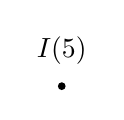
\begin{tikzpicture}[baseline=-2pt]\fill (0,0) circle (1.4pt);\node[above] at (0,.15) {$I(5)$};\end{tikzpicture}}\xrightarrow{(10)}&
\figure{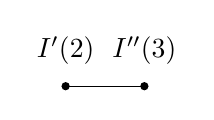
\begin{tikzpicture}[baseline=-2pt]\draw (0,0)--(1,0);\fill (0,0) circle (1.5pt);\fill (1,0) circle (1.5pt);\node[above] at (0,.15) {$I'(2)$};\node[above] at (1,.15) {$I''(3)$};\end{tikzpicture}}\xrightarrow{(3)}&
\figure{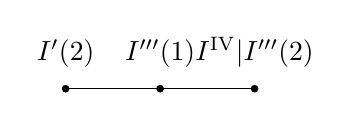
\begin{tikzpicture}[baseline=-2pt]\draw (0,0)--(1.2,0)--(2.4,0);\foreach \x in {0,1.2,2.4}{\fill (\x,0) circle (1.4pt);}\node[above] at (0,.15) {$I'(2)$};\node[above] at (1.2,.15) {$I'''(1)$};\node[above] at (2.4,.15) {$\unsure{I^{\mathrm{IV}}|I'''}(2)$};\end{tikzpicture}}
\end{array}}
\]
Dans $\widehat M^!_{0,5}$ il y a dix ``diviseurs à l'infini'' \inserted{$(I'(2),I'')$}, dont chacun est un $\widehat M^!_{0,4}$ \deleted{\unsure{$\simeq\mathbf P$}}, \deleted{\unsure{$\mathbf P^1_{0,3}\mathfrak S_3$}} \inserted{(plus précisément, un $\widehat M_{0,I''(3)\amalg(*)}\simeq(\mathbf P^1_{I''})_{\mathbf Z}$)} (ayant comme on avait vu, et \unsure{avait|aurait}) trois points à l'infini --- les pts à l'infini sont en nb total $\frac{30}{2}=15$, correspondant aux partitions de $I(5)$ de type $(2,2,1)$, alors que les diviseurs à l'infini correspondent aux parties \inserted{$I'$} de $I$ de cardinal $2$. Deux tels diviseurs, correspondant à des parties $I',I''\in\mathfrak P_2(I)$, se rencontrent sss \deleted{elles} on a $I'\cap I''=\varnothing$, i.e. si $I',I''$ et $I\smallsetminus(I'\cup I'')$ forment justement une partition de $I$ de type $(2,2,1)$.
\margin{$\mathbf P^1_{I''}\overset{\mathrm{déf}}=\unsure{\mathbf P^1_{\mathbf Z}\wedge_{\mathfrak S_3}\widetilde{I''}}$}

D'après l'étude combinatoire de l'\unsure{icosaèdre}, choisissant une orientation de $I$ --- ce qui détermine un \unsure{icosaèdre} orienté, ou encore un icos. graphe) les $10$ diviseurs à l'infini de $\widehat M_{0,I}$, i.e. les \inserted{$10$} éléments de $\mathfrak P_2(I)$, \deleted{\unsure{en ordre}} \inserted{ou (par} \deleted{\unsure{correspon-}}
\margin{65}
